\section{Problem Description}\label{sec:prob_descr}
The problems revolves around a physical system of a helicopter arm which is fasten to the ground and has three degrees of freedom. Elevation ($e$), pitch ($p$) and travel ($\lambda$). 
The helicopter was controlled through a joystick and interfaced to the helicopter with \MATLAB. The following tasks are described in the report:

\begin{itemize}
    \item Derive a mathematical model for the system.
    \item Derive and apply PD and multivariable controllers for the system.
    \item Estimate states that are not directly measured.
    \item Develop a linear quadratic regulator (LQR) for the system.
\end{itemize}

The helicopter can be modeled as three point masses: two masses represent the motors of the propellers and the third is the counterweight on the opposite side. Refer to figure~\ref{fig:heli} for depiction of setup. The cynlindres of figure~\ref{fig:heli} are the joints where the axis of the cylindres are equal to the axis of rotation of the joint. The following definitions are made: \textit{p} is the pitch angle of the helicopter head, \textit{e} is denotes its elevation angle and \textit{$\lambda$} denotes the travel angle of the helicopter. Figure \ref{fig:heli} shows all angles at zero and with positive orientation as indicated. For the sake of this report, it is assumed that there is a linear relationship between the forces the propellers generate and the voltage that is applied to them:

\begin{subequations}\label{eq:P1_forces_propellers}
    \begin{align}
        F_f&=K_f V_f     \label{eq:P1_forces_propellers_f} \\
        F_b&=K_b V_b     \label{eq:P1_forces_propellers_b}
    \end{align}
\end{subequations}

The propellers are placed symmetrically in relation to the pitch axis and the forces always attack perpendicular to the plane made by the pitch and elevation axis. The weight of the the point masses are called $F_{g,f}, F_{g,b}$ and $F_{g,c}$ and attack parallel to gravity.

For the sake of this report, it is assumed that the weight of the two propeller motors are equal and given by $m_p$. The counterweight mass is indicated by $m_c$. The distance along the elevation axis between the travel axis and pitch axis is indicated by $l_h$. The length from the travel axis to the counterweight is indicated by $l_c$. 

\begin{figure}[bp]
	\centering
	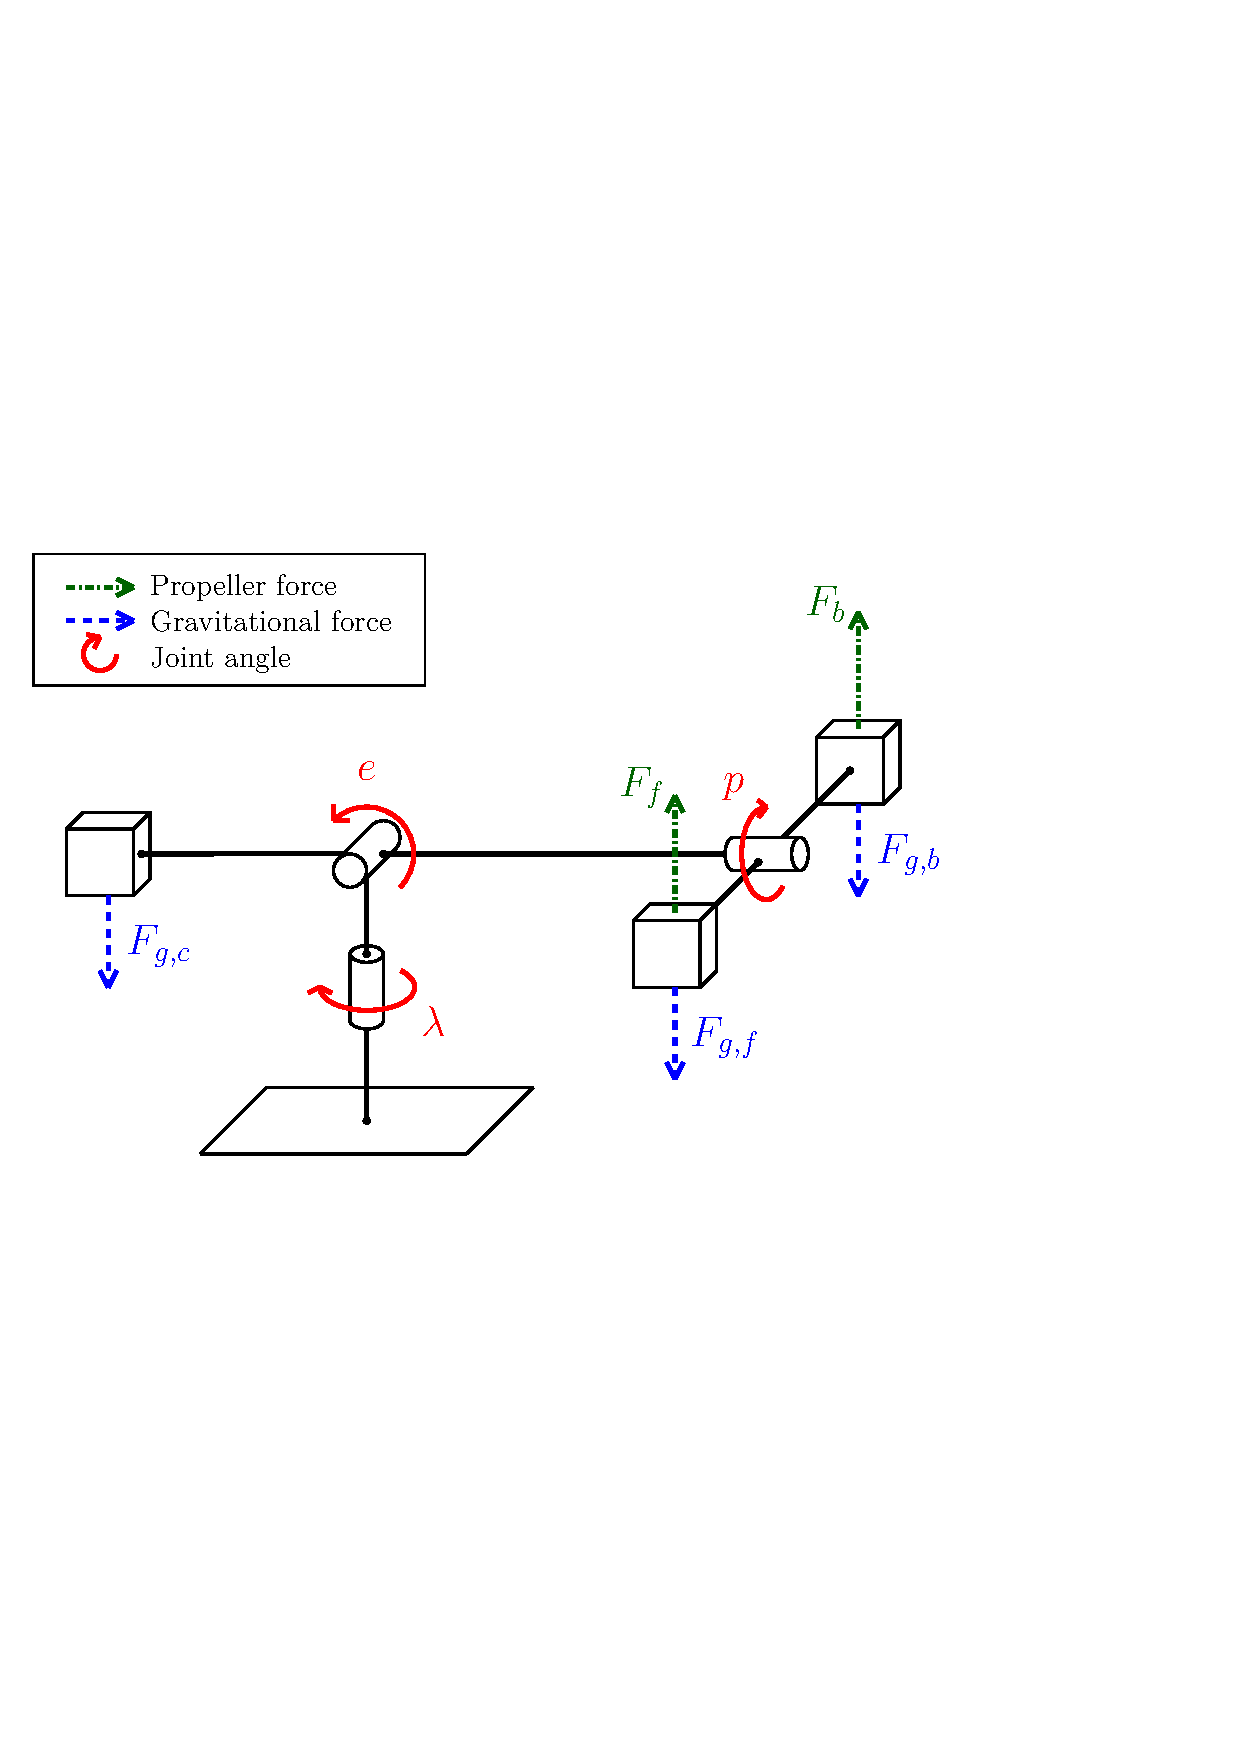
\includegraphics[width=0.80\textwidth]{figures/forces.pdf}
	\caption{Depiction of model of system.}
\label{fig:heli}
\end{figure}

The report is divided into four parts. The first part will make mathematical descriptions of the described system. Part II will describe the implementation of monovariable control through the use of PD and P controllers. Part III will describe the implementation of an LQR controller and lastly, Part IV will describe the implementation of a state estimation model into the LQR controller.
